%% generato automaticamente da tools/build_tex.py --- non modificare
\chapter{Il quaderno grande}
\label{cap:mate}
\quaderno{mate.dfw}{18 Aug 2010}{133}

Agosto 2010, centotrentatré espressioni: è il file più lungo della raccolta e quello che più somiglia a un taccuino nel senso proprio del termine. Non ha un argomento unico; ha invece dieci filoni che si susseguono, alcuni chiusi in poche righe, altri ripresi decine di espressioni più avanti. Il filo conduttore, se c'è, è la ricerca di identità esatte nascoste dietro espressioni che sembrano dipendere da tutto: rapporti che valgono una costante qualunque siano gli argomenti, funzioni non elementari costruite con soli logaritmi e valori assoluti, onde triangolari fabbricate con arcocoseni.

\section{L'identità del mezzo}

Il quaderno si apre con la sua ossessione principale, e la prima riga è quasi uno scherzo: un rapporto identico a sé stesso vale uno. La seconda è invece l'identità vera, quella che tornerà una quarantina di volte nelle pagine seguenti.

\begin{espr}{1}{User}{\verificata}
\[
\frac{\cos\!\left(x\right) - \cos\!\left(y\right)}{\cos\!\left(x\right) - \cos\!\left(y\right)} = 1
\]
\end{espr}
Un rapporto identico a sé stesso. Sembra banale ma fissa lo schema: numeratore e denominatore costruiti sugli stessi due argomenti.

\begin{espr}{2}{User}{\verificata}
\[
\frac{\cos^{2}\!\left(x\right) - \cos^{2}\!\left(y\right)}{\cos\!\left(2\, x\right) - \cos\!\left(2\, y\right)} = \frac{1}{2}
\]
\end{espr}
L'identità centrale del quaderno. Conseguenza immediata di $\cos2\theta=2\cos^2\theta-1$.

\begin{espr}{3}{User}{\verificata}
\[
\frac{\cosh^{2}\!\left(x\right) - \cosh^{2}\!\left(y\right)}{\cosh\!\left(2\, x\right) - \cosh\!\left(2\, y\right)} = \frac{1}{2}
\]
\end{espr}
La stessa cosa con il coseno iperbolico, che soddisfa la formula di duplicazione con gli stessi coefficienti.

\begin{espr}{4}{User}{\verificata}
\[
\frac{\sin^{2}\!\left(x\right) - \sin^{2}\!\left(y\right)}{\cos\!\left(2\, x\right) - \cos\!\left(2\, y\right)} = -\frac{1}{2}
\]
\end{espr}
Con i seni il segno si rovescia, perché $\sin^2\theta=(1-\cos2\theta)/2$.

\begin{espr}{5}{User}{\verificata}
\begin{align*}
& \frac{\cos^{3}\!\left(x\right)\, \cos\!\left(y\right) - \cos^{3}\!\left(y\right)\, \cos\!\left(x\right)}{\cos\!\left(3\, x\right)\, \cos\!\left(y\right) - \cos\!\left(3\, y\right)\, \cos\!\left(x\right)} \\
=\;& \frac{\cos\!\left(x\right)\, \cos\!\left(y\right)\, \left(\cos^{2}\!\left(x\right) - \cos^{2}\!\left(y\right)\right)}{\cos\!\left(y\right)\, \cos\!\left(3\, x\right) - \cos\!\left(x\right)\, \cos\!\left(3\, y\right)} \\
=\;& \frac{1}{4}
\end{align*}
\end{espr}
La versione al terzo grado, che dà $1/4$. Il coefficiente viene dal $4$ di $\cos3\theta=4\cos^3\theta-3\cos\theta$.

\begin{espr}{6}{User}{\verificata}
\begin{align*}
& \frac{\mathrm{e}^{2\, \mathrm{i}\, x} - \mathrm{e}^{2\, \mathrm{i}\, y} + \sin^{2}\!\left(y\right) - \sin^{2}\!\left(x\right) + 2\, \mathrm{i}\, \left(\mathrm{e}^{\mathrm{i}\, y}\, \sin\!\left(y\right) - \mathrm{e}^{\mathrm{i}\, x}\, \sin\!\left(x\right)\right)}{\mathrm{e}^{2\, \mathrm{i}\, x} - \mathrm{e}^{2\, \mathrm{i}\, y} + \mathrm{i}\, \left(\sin\!\left(2\, y\right) - \sin\!\left(2\, x\right)\right)} \\
=\;& \frac{1}{2}
\end{align*}
\end{espr}
La stessa identità riscritta con esponenziali complessi.

\begin{espr}{7}{User}{}
\begin{align*}
& \operatorname{Re}\!\left(\mathrm{e}^{2\, \mathrm{i}\, x} - \mathrm{e}^{2\, \mathrm{i}\, y} + \mathrm{i}\, \left(\sin\!\left(2\, y\right) - \sin\!\left(2\, x\right)\right)\right) \\
=\;& \cos\!\left(2\, x\right) - \cos\!\left(2\, y\right)
\end{align*}
\end{espr}
Verifica che la parte reale del denominatore sia quella attesa.

\begin{espr}{8}{User}{}
\begin{align*}
& \operatorname{Im}\!\left(\mathrm{e}^{2\, \mathrm{i}\, x} - \mathrm{e}^{2\, \mathrm{i}\, y} + \mathrm{i}\, \left(\sin\!\left(2\, y\right) - \sin\!\left(2\, x\right)\right)\right) \\
=\;& 0
\end{align*}
\end{espr}
E che la parte immaginaria si annulli.

\begin{espr}{9}{User}{}
\begin{align*}
& \operatorname{Re}\!\left(\mathrm{e}^{2\, \mathrm{i}\, x} - \mathrm{e}^{2\, \mathrm{i}\, y} + \sin^{2}\!\left(y\right) - \sin^{2}\!\left(x\right) + 2\, \mathrm{i}\, \left(\mathrm{e}^{\mathrm{i}\, y}\, \sin\!\left(y\right) - \mathrm{e}^{\mathrm{i}\, x}\, \sin\!\left(x\right)\right)\right) \\
=\;& \frac{\cos\!\left(2\, x\right)}{2} - \frac{\cos\!\left(2\, y\right)}{2}
\end{align*}
\end{espr}
Idem per il numeratore, che dà metà.

\begin{espr}{10}{User}{}
\begin{align*}
& \operatorname{Im}\!\left(\mathrm{e}^{2\, \mathrm{i}\, x} - \mathrm{e}^{2\, \mathrm{i}\, y} + \sin^{2}\!\left(y\right) - \sin^{2}\!\left(x\right) + 2\, \mathrm{i}\, \left(\mathrm{e}^{\mathrm{i}\, y}\, \sin\!\left(y\right) - \mathrm{e}^{\mathrm{i}\, x}\, \sin\!\left(x\right)\right)\right) \\
=\;& 0
\end{align*}
\end{espr}
E la sua parte immaginaria è nulla.

\begin{espr}{11}{User}{\verificata}
\begin{align*}
& \cos\!\left(5\, x\right) \\
=\;& \left(\cos\!\left(x\right)\, \cos\!\left(2\, x\right) - \sin\!\left(x\right)\, \sin\!\left(2\, x\right)\right)\, \cos\!\left(2\, x\right) - \sin\!\left(2\, x\right)\, \left(\sin\!\left(x\right)\, \cos\!\left(2\, x\right) + \sin\!\left(2\, x\right)\, \cos\!\left(x\right)\right)
\end{align*}
\end{espr}
Il coseno di $5x$ ottenuto componendo due volte le formule di addizione.

\begin{espr}{12}{User}{\verificata}
\[
\cos\!\left(5\, x\right) = \cos\!\left(x\right)\, \cos\!\left(4\, x\right) - \sin\!\left(x\right)\, \sin\!\left(4\, x\right)
\]
\end{espr}
Lo stesso in un passaggio solo. Le due righe verificano la coerenza dello sviluppo.


La dimostrazione sta nella formula di duplicazione. Da $\cos2\theta=2\cos^2\theta-1$ segue $\cos2x-\cos2y=2\left(\cos^2x-\cos^2y\right)$: il rapporto vale $1/2$ per ogni $x$ e ogni $y$ per cui il denominatore non si annulla, e il fatto che sia costante non dipende da nulla. La riga $\#3$ osserva che la stessa cosa vale per il coseno iperbolico, perché $\cosh2\theta=2\cosh^2\theta-1$ ha la stessa forma. La riga $\#4$ fa il conto con i seni e trova $-1/2$, perché $\sin^2\theta=(1-\cos2\theta)/2$ inverte il segno.

La riga $\#5$ è il salto interessante: la stessa costruzione al terzo grado. Da $\cos3\theta=4\cos^3\theta-3\cos\theta$ segue che $\cos^3x\cos y-\cos^3y\cos x$ vale esattamente un quarto di $\cos3x\cos y-\cos3y\cos x$, perché i termini in $-3\cos$ si cancellano fra loro. Duplicazione dà $1/2$, triplicazione dà $1/4$: in entrambi i casi la costante è il reciproco del coefficiente direttivo del polinomio di Chebyshev, $2^{1-n}$. La regola vale solo per $n=2$ e $n=3$, però: dal quarto grado in poi il polinomio di Chebyshev ha due termini di grado inferiore, e una combinazione di due soli coseni non basta più a eliminarli. Con più angoli, invece, la regola vale per ogni $n$ come identità fra determinanti: lo mostra la nota a corredo di questa edizione.

\section{Due unità immaginarie e un seno cardinale}

Un breve intermezzo su un sistema di tre equazioni e su alcune varianti del seno cardinale.

\begin{espr}{13}{Solve(User,[f,m,s])}{}
\[
\operatorname{Solve}\!\left(\left[\, f^{2} + m^{2} = 0,\; f\, m = 1,\; s = \frac{1}{2}\, \left(f + m\right) \,\right],\; \left[\, f,\; m,\; s \,\right]\right)
\]
\end{espr}
Un sistema: due numeri con somma dei quadrati nulla e prodotto unitario.

\begin{espr}{14}{Simp(Solve(User,[f,m,s]))}{}
\[
\left[\, f = \frac{\sqrt{2}}{2} + \frac{\sqrt{2}\, \mathrm{i}}{2} \;\land\; m = \frac{\sqrt{2}}{2} - \frac{\sqrt{2}\, \mathrm{i}}{2} \;\land\; s = \frac{\sqrt{2}}{2},\; f = \frac{\sqrt{2}}{2} - \frac{\sqrt{2}\, \mathrm{i}}{2} \;\land\; m = \frac{\sqrt{2}}{2} + \frac{\sqrt{2}\, \mathrm{i}}{2} \;\land\; s = \frac{\sqrt{2}}{2},\; f = -\frac{\sqrt{2}}{2} + \frac{\sqrt{2}\, \mathrm{i}}{2} \;\land\; m = -\frac{\sqrt{2}}{2} - \frac{\sqrt{2}\, \mathrm{i}}{2} \;\land\; s = -\frac{\sqrt{2}}{2},\; f = -\frac{\sqrt{2}}{2} - \frac{\sqrt{2}\, \mathrm{i}}{2} \;\land\; m = -\frac{\sqrt{2}}{2} + \frac{\sqrt{2}\, \mathrm{i}}{2} \;\land\; s = -\frac{\sqrt{2}}{2} \,\right]
\]
\end{espr}
Le quattro soluzioni sono le radici ottave dell'unità sulle bisettrici; la semisomma vale $\pm\sqrt2/2$.

\begin{espr}{15}{User}{}
\[
\frac{n\, \sin^{x}\!\left(\pi\, x\right)}{\pi\, x}
\]
\end{espr}
Una variante del seno cardinale con esponente variabile.

\begin{espr}{16}{User}{}
\[
\frac{\sin\!\left(\mathrm{e}\, x\right)}{\mathrm{e}\, x}
\]
\end{espr}
Il seno cardinale con pulsazione $\mathrm{e}$.

\begin{espr}{17}{User}{}
\[
\frac{n\, \sin\!\left(\mathrm{e}\, x\right)}{\mathrm{e}\, x}
\]
\end{espr}
Moltiplicato per un fattore che tende all'infinito.

\begin{espr}{18}{User}{}
\[
\lim_{n \to \infty} \frac{n\, \sin\!\left(\mathrm{e}\, x\right)}{\mathrm{e}\, x}
\]
\end{espr}
Il limite diverge ovunque tranne che negli zeri del seno: l'espressione non ha limite come funzione.


Il sistema $\#13$ chiede due numeri il cui quadrato sommato faccia zero e il cui prodotto faccia uno. Da $f^2+m^2=0$ e $fm=1$ segue $(f+m)^2=2fm=2$, quindi la semisomma vale $\pm\sqrt2/2$: sono le quattro radici ottave dell'unità che stanno sulle bisettrici, cioè $(\pm1\pm\mathrm{i})/\sqrt2$.

\section{La caccia al parametro}

Trenta espressioni dedicate a una sola domanda, posta e riposta in sei varianti: se nell'identità del mezzo si sostituisce $y$ con $ky$, per quale $k$ l'identità continua a valere? La risposta di Derive è sempre la stessa, ed è un numero che sembra dire qualcosa.

\begin{espr}{19}{User}{}
\[
\frac{\cos^{2}\!\left(x + \mathrm{i}\, y\right) - \cos^{2}\!\left(x - \mathrm{i}\, y\right)}{\cos\!\left(2\, x + 2\, \mathrm{i}\, y\right) - \cos\!\left(2\, x - 2\, \mathrm{i}\, y\right)}
\]
\end{espr}
L'identità con argomenti complessi coniugati $x\pm\mathrm{i}y$.

\begin{espr}{20}{Simp(\#19)}{}
\[
\frac{1}{2}
\]
\end{espr}
Vale ancora $1/2$: l'identità è algebrica e non distingue reale da complesso.

\begin{espr}{21}{User}{\verificata}
\begin{align*}
& \frac{\cos^{2}\!\left(x + k\, y\right) - \cos^{2}\!\left(x - k\, y\right)}{\cos\!\left(2\, x + 2\, k\, y\right) - \cos\!\left(2\, x - 2\, k\, y\right)} \\
=\;& \frac{1}{2}
\end{align*}
\end{espr}
Si sostituisce $\mathrm{i}$ con un parametro $k$ generico.

\begin{espr}{22}{Solve(\#21,k)}{}
\[
\operatorname{Approx}\!\left(\operatorname{Solve}\!\left(\frac{\cos^{2}\!\left(x + k\, y\right) - \cos^{2}\!\left(x - k\, y\right)}{\cos\!\left(2\, x + 2\, k\, y\right) - \cos\!\left(2\, x - 2\, k\, y\right)} = \frac{1}{2},\; k\right)\right)
\]
\end{espr}
Si chiede a Derive di risolvere numericamente rispetto a $k$.

\begin{espr}{23}{Simp(Solve(\#21,k))}{}
\[
k = -4.999999701
\]
\end{espr}
La risposta. È il punto in cui si è fermata l'iterazione, non una soluzione: l'equazione è soddisfatta da ogni $k$.

\begin{espr}{24}{User}{\verificata}
\begin{align*}
& \frac{\cos^{2}\!\left(x + \mathrm{i}\, y\right) - \cos^{2}\!\left(x - \mathrm{i}\, y\right)}{\cos\!\left(2\, x + 2\, \mathrm{i}\, y\right) - \cos\!\left(2\, x - 2\, \mathrm{i}\, y\right)} \\
=\;& \frac{1}{2}
\end{align*}
\end{espr}
L'identità con $\mathrm{i}$, ripetuta per confronto.

\begin{espr}{25}{User}{\verificata}
\begin{align*}
& \frac{\cos^{2}\!\left(x + k\, y\right) - \cos^{2}\!\left(k\, y\right)}{\cos\!\left(2\, x + 2\, k\, y\right) - \cos\!\left(2\, k\, y\right)} \\
=\;& \frac{1}{2}
\end{align*}
\end{espr}
Variante: il secondo argomento perde la $x$.

\begin{espr}{26}{Solve(\#25,k)}{}
\[
\operatorname{Approx}\!\left(\operatorname{Solve}\!\left(\frac{\cos^{2}\!\left(x + k\, y\right) - \cos^{2}\!\left(k\, y\right)}{\cos\!\left(2\, x + 2\, k\, y\right) - \cos\!\left(2\, k\, y\right)} = \frac{1}{2},\; k\right)\right)
\]
\end{espr}
Stessa domanda.

\begin{espr}{27}{Simp(Solve(\#25,k))}{}
\[
k = -4.999999701
\]
\end{espr}
Stessa risposta, il che conferma che il numero dipende dal risolutore e non dall'equazione.

\begin{espr}{28}{User}{\verificata}
\[
\frac{\cos^{2}\!\left(3\, x + k\, y\right) - \cos^{2}\!\left(x\right)}{\cos\!\left(6\, x + 2\, k\, y\right) - \cos\!\left(2\, x\right)} = \frac{1}{2}
\]
\end{espr}
Variante con argomenti $3x+ky$ e $x$.

\begin{espr}{29}{Solve(\#28,k)}{}
\[
\operatorname{Approx}\!\left(\operatorname{Solve}\!\left(\frac{\cos^{2}\!\left(3\, x + k\, y\right) - \cos^{2}\!\left(x\right)}{\cos\!\left(6\, x + 2\, k\, y\right) - \cos\!\left(2\, x\right)} = \frac{1}{2},\; k\right)\right)
\]
\end{espr}
Stessa domanda.

\begin{espr}{30}{Simp(\#29)}{}
\[
k = -4.999999701
\]
\end{espr}
Stessa risposta.

\begin{espr}{31}{User}{\verificata}
\[
\frac{\cos^{2}\!\left(x + k\right) - \cos^{2}\!\left(x - k\right)}{\cos\!\left(2\, x + 2\, k\right) - \cos\!\left(2\, x - 2\, k\right)} = \frac{1}{2}
\]
\end{espr}
Variante senza $y$.

\begin{espr}{32}{Solve(\#31,k)}{}
\[
\operatorname{Approx}\!\left(\operatorname{Solve}\!\left(\frac{\cos^{2}\!\left(x + k\right) - \cos^{2}\!\left(x - k\right)}{\cos\!\left(2\, x + 2\, k\right) - \cos\!\left(2\, x - 2\, k\right)} = \frac{1}{2},\; k,\; \mathrm{Real}\right)\right)
\]
\end{espr}
Stessa domanda, questa volta limitata alle soluzioni reali.

\begin{espr}{33}{Simp(Solve(\#31,k))}{}
\[
k = -4.999999701
\]
\end{espr}
Stessa risposta.

\begin{espr}{34}{User}{\verificata}
\begin{align*}
& \frac{\cos^{3}\!\left(x\right)\, \cos\!\left(y\right) - \cos^{3}\!\left(y\right)\, \cos\!\left(x\right)}{\cos\!\left(3\, x\right)\, \cos\!\left(y\right) - \cos\!\left(3\, y\right)\, \cos\!\left(x\right)} \\
=\;& \frac{\cos\!\left(x\right)\, \cos\!\left(y\right)\, \left(\cos^{2}\!\left(x\right) - \cos^{2}\!\left(y\right)\right)}{\cos\!\left(y\right)\, \cos\!\left(3\, x\right) - \cos\!\left(x\right)\, \cos\!\left(3\, y\right)} \\
=\;& \frac{1}{4}
\end{align*}
\end{espr}
L'identità al quarto, ripresa dalla riga $\#5$.

\begin{espr}{35}{User}{\verificata}
\begin{align*}
& \frac{\cos\!\left(x + k\, y\right)\, \cos\!\left(x - k\, y\right)\, \left(\cos^{2}\!\left(x + k\, y\right) - \cos^{2}\!\left(x - k\, y\right)\right)}{\cos\!\left(x - k\, y\right)\, \cos\!\left(3\, x + 3\, k\, y\right) - \cos\!\left(x + k\, y\right)\, \cos\!\left(3\, x - 3\, k\, y\right)} \\
=\;& \frac{1}{4}
\end{align*}
\end{espr}
La sua versione con il parametro.

\begin{espr}{36}{Solve(\#35,k)}{}
\[
\operatorname{Approx}\!\left(\operatorname{Solve}\!\left(\frac{\cos\!\left(x + k\, y\right)\, \cos\!\left(x - k\, y\right)\, \left(\cos^{2}\!\left(x + k\, y\right) - \cos^{2}\!\left(x - k\, y\right)\right)}{\cos\!\left(x - k\, y\right)\, \cos\!\left(3\, x + 3\, k\, y\right) - \cos\!\left(x + k\, y\right)\, \cos\!\left(3\, x - 3\, k\, y\right)} = \frac{1}{4},\; k\right)\right)
\]
\end{espr}
Si chiede $k$.

\begin{espr}{37}{Simp(Solve(\#35,k))}{}
\[
k = 0
\]
\end{espr}
La risposta $k=0$ corrisponde al caso in cui numeratore e denominatore si annullano entrambi.

\begin{espr}{38}{User}{}
\[
\frac{\cos\!\left(x\right)\, \cos\!\left(y\right)\, \left(\cos^{2}\!\left(x\right) - \cos^{2}\!\left(y\right)\right)}{\cos\!\left(y\right)\, \cos\!\left(3\, x\right) - \cos\!\left(x\right)\, \cos\!\left(3\, y\right)}
\]
\end{espr}
Il primo membro isolato.

\begin{espr}{39}{User}{\verificata}
\begin{align*}
& \frac{\cos^{2}\!\left(x + k\, y\right) - \cos^{2}\!\left(x - k\, y\right)}{\cos\!\left(2\, x + 2\, k\, y\right) - \cos\!\left(2\, x - 2\, k\, y\right)} \\
=\;& \frac{1}{2}
\end{align*}
\end{espr}
L'equazione ripetuta.

\begin{espr}{40}{User}{\verificata}
\begin{align*}
& \frac{\cos^{2}\!\left(x - 4.999999701\, y\right) - \cos^{2}\!\left(x + 4.999999701\, y\right)}{\cos\!\left(2\, x - 2 \cdot 4.999999701\, y\right) - \cos\!\left(2\, x + 2 \cdot 4.999999701\, y\right)} \\
=\;& \frac{1}{2}
\end{align*}
\end{espr}
Il valore numerico sostituito esplicitamente al posto di $k$, per verifica.

\begin{espr}{41}{User}{\verificata}
\[
\frac{\cos^{2}\!\left(x\right) - \cos^{2}\!\left(y\right)}{\cos\!\left(2\, x\right) - \cos\!\left(2\, y\right)} = \frac{1}{2}
\]
\end{espr}
L'identità nella forma originale.

\begin{espr}{42}{User}{\verificata}
\[
\frac{\cos^{2}\!\left(x + y\right) - \cos^{2}\!\left(x - y\right)}{\cos\!\left(2\, x + 2\, y\right) - \cos\!\left(2\, x - 2\, y\right)} = \frac{1}{2}
\]
\end{espr}
Con $k=1$, cioè argomenti $x\pm y$: vale ancora.

\begin{espr}{43}{Simp(Solve(User,y))}{}
\[
y = -4.999999701
\]
\end{espr}
E ancora lo stesso numero, ora attribuito a $y$.

\begin{espr}{44}{User}{\verificata}
\begin{align*}
& \frac{\cos\!\left(x + y\right)\, \cos\!\left(x - y\right)\, \left(\cos^{2}\!\left(x + y\right) - \cos^{2}\!\left(x - y\right)\right)}{\cos\!\left(x - y\right)\, \cos\!\left(3\, x + 3\, y\right) - \cos\!\left(x + y\right)\, \cos\!\left(3\, x - 3\, y\right)} \\
=\;& \frac{1}{4}
\end{align*}
\end{espr}
La versione al quarto con $k=1$.

\begin{espr}{45}{User}{}
\[
y = -2.499998615
\]
\end{espr}
Un valore numerico circa la metà del precedente.

\begin{espr}{46}{User}{}
\[
k\, 3.141592654 = -4.999999701
\]
\end{espr}
Il tentativo di interpretazione: si divide il numero per $\pi$.

\begin{espr}{47}{Solve(\#46,k)}{}
\[
\operatorname{Approx}\!\left(\operatorname{Solve}\!\left(k\, 3.141592654 = -4.999999701,\; k,\; \mathrm{Real}\right)\right)
\]
\end{espr}
La divisione.

\begin{espr}{48}{Simp(Solve(\#46,k))}{}
\[
k = -1.591549335
\]
\end{espr}
Il risultato è $-5/\pi=-1{,}5915494$, il che era prevedibile visto che il numeratore era $-5$ a meno di tre decimilionesimi.


Qui conviene fermarsi, perché la risposta è una trappola e vale la pena di riconoscerla.

L'identità $\left(\cos^2 u-\cos^2 v\right)/\left(\cos 2u-\cos 2v\right)=1/2$ vale per \emph{ogni} coppia di argomenti. Ponendo $u=x+ky$ e $v=x-ky$ si ottiene dunque un'uguaglianza vera per \emph{ogni} $k$: l'equazione $\#21$ non ha una soluzione, ne ha infinite, ed è quindi indeterminata. Quando le si chiede di risolverla numericamente, Derive avvia una ricerca di zeri su una funzione identicamente nulla e restituisce il punto in cui l'iterazione si è fermata. Quel punto è $-4{,}999999701$, e non ha alcun significato matematico: cambiando il punto di partenza cambierebbe.

Il quaderno prende però quel numero sul serio e prova a interpretarlo. Alla riga $\#46$ lo divide per $\pi$ e ottiene $-1{,}591549335$, che è $-5/\pi$ con sette cifre esatte — inevitabilmente, visto che il numero di partenza è $-5$ a meno di tre decimilionesimi. È il tipo di inseguimento che ogni tanto capita di fare, e questa raccolta lo conserva senza correggerlo: fa parte del documento.

Analoga osservazione per la riga $\#37$, dove Derive risponde $k=0$ alla versione al quarto: in $k=0$ numeratore e denominatore si annullano entrambi, e la risposta segnala una forma indeterminata più che una soluzione.

\section{La stessa identità con due parametri}

La domanda viene riformulata in un modo che finalmente non è degenere: si introducono due parametri, uno al numeratore e uno al denominatore, e si chiede quale relazione debbano soddisfare.

\begin{espr}{49}{User}{\verificata}
\[
\frac{\cos^{2}\!\left(x\right) - \cos^{2}\!\left(y\right)}{\cos\!\left(2\, x\right) - \cos\!\left(2\, y\right)} = \frac{1}{2}
\]
\end{espr}
Si riparte dall'identità.

\begin{espr}{50}{User}{}
\[
\cos^{2}\!\left(x\right) - \cos^{2}\!\left(y\right) = 1
\]
\end{espr}
Si impone che il numeratore valga $1$...

\begin{espr}{51}{User}{}
\[
\cos\!\left(2\, x\right) - \cos\!\left(2\, y\right) = 2
\]
\end{espr}
...e il denominatore $2$.

\begin{espr}{52}{Solve(User,[j,k])}{}
\[
\operatorname{Solve}\!\left(\left[\, \cos^{2}\!\left(k\right) - \cos^{2}\!\left(j\right) = 1,\; \cos\!\left(2\, k\right) - \cos\!\left(2\, j\right) = 2 \,\right],\; \left[\, j,\; k \,\right]\right)
\]
\end{espr}
Il sistema corrispondente. Non ha soluzioni reali: $\cos^2k-\cos^2j=1$ richiede $\cos k=\pm1$ e $\cos j=0$, ma allora la seconda equazione dà $2$ soltanto con segni concordi.

\begin{espr}{53}{User}{}
\[
\frac{\cos^{2}\!\left(x\right) - k\, \cos^{2}\!\left(y\right)}{\cos\!\left(2\, x\right) - l\, \cos\!\left(2\, y\right)} = \frac{1}{2}
\]
\end{espr}
La generalizzazione con due parametri: ora l'identità non è più automatica.

\begin{espr}{54}{Simp(Solve(\#53,k))}{}
\[
k = \frac{l\, \cos\!\left(2\, y\right) + 1}{2\, \cos^{2}\!\left(y\right)}
\]
\end{espr}
Risolta rispetto a $k$.

\begin{espr}{55}{Simp(Solve(\#53,l))}{}
\[
l = \frac{2\, k\, \cos^{2}\!\left(y\right) - 1}{\cos\!\left(2\, y\right)}
\]
\end{espr}
E rispetto a $l$.

\begin{espr}{56}{User}{}
\[
\operatorname{Solve}\!\left(\left[\, k = \frac{l\, \cos\!\left(2\, y\right) + 1}{2\, \cos^{2}\!\left(y\right)},\; l = \frac{2\, k\, \cos^{2}\!\left(y\right) - 1}{\cos\!\left(2\, y\right)} \,\right],\; \left[\, k,\; l \,\right]\right)
\]
\end{espr}
Si chiede quando le due relazioni siano simultaneamente vere.

\begin{espr}{57}{Simp(Solve(User,[k,l]))}{}
\[
\left[\, \frac{\left(k - l\right)\, \cos\!\left(2\, y\right) + k}{\cos\!\left(2\, y\right) + 1} = \frac{1}{\cos\!\left(2\, y\right) + 1} \,\right]
\]
\end{espr}
La risposta è una sola equazione: il sistema è degenere e le soluzioni formano una curva.

\begin{espr}{58}{Solve(\#57,k)}{}
\[
\operatorname{Solve}\!\left(\left[\, \frac{\left(k - l\right)\, \cos\!\left(2\, y\right) + k}{\cos\!\left(2\, y\right) + 1} = \frac{1}{\cos\!\left(2\, y\right) + 1} \,\right],\; k\right)
\]
\end{espr}
Si prova a isolare $k$.

\begin{espr}{59}{Simp(Solve(\#57,k))}{}
\[
\left[\, k = \frac{l\, \cos\!\left(2\, y\right) + 1}{\cos\!\left(2\, y\right) + 1} \,\right]
\]
\end{espr}
La relazione finale.

\begin{espr}{60}{User}{}
\[
\cos\!\left(2\, y\right) = \frac{1 - k}{k - l}
\]
\end{espr}
Riscritta in modo da esprimere $\cos2y$.

\begin{espr}{61}{User}{}
\begin{align*}
& \frac{\cos^{2}\!\left(x\right) - x\, \left(1 + k\right)\, \cos^{2}\!\left(y\right)}{\cos\!\left(2\, x\right) - y\, \left(1 + k\right)\, \cos\!\left(2\, y\right)} \\
=\;& \frac{1}{2}
\end{align*}
\end{espr}
Una variante con i parametri intrecciati alle variabili.

\begin{espr}{62}{Simp(Solve(\#61,k))}{}
\[
k = -\frac{\left(x - y\right)\, \cos\!\left(2\, y\right) + x - 1}{\left(x - y\right)\, \cos\!\left(2\, y\right) + x}
\]
\end{espr}
La soluzione corrispondente.

\begin{espr}{63}{User}{}
\begin{align*}
& \frac{\cos^{2}\!\left(x\right) - \left(1 + k\right)\, \cos^{2}\!\left(y\right)}{\cos\!\left(2\, x\right) - \left(1 + k\right)\, \cos\!\left(2\, y\right)} \\
=\;& \frac{k}{2}
\end{align*}
\end{espr}
La formulazione più ricca: anche il secondo membro dipende da $k$.

\begin{espr}{64}{Solve(\#63,k)}{}
\[
\operatorname{Solve}\!\left(\frac{\cos^{2}\!\left(x\right) - \left(1 + k\right)\, \cos^{2}\!\left(y\right)}{\cos\!\left(2\, x\right) - \left(1 + k\right)\, \cos\!\left(2\, y\right)} = \frac{k}{2},\; k\right)
\]
\end{espr}
La richiesta.

\begin{espr}{65}{Simp(Solve(\#63,k))}{}
\begin{align*}
& k = -\frac{\sqrt{\cos^{2}\!\left(2\, x\right) + 2\, \cos\!\left(2\, x\right)\, \left(1 - 2\, \cos\!\left(2\, y\right)\right) + 4\, \cos^{2}\!\left(2\, y\right) + 1}}{2\, \cos\!\left(2\, y\right)} + \frac{\cos\!\left(2\, x\right)}{2\, \cos\!\left(2\, y\right)} + \frac{1}{2\, \cos\!\left(2\, y\right)} \\[3pt]
\lor\quad & k = \frac{\sqrt{\cos^{2}\!\left(2\, x\right) + 2\, \cos\!\left(2\, x\right)\, \left(1 - 2\, \cos\!\left(2\, y\right)\right) + 4\, \cos^{2}\!\left(2\, y\right) + 1}}{2\, \cos\!\left(2\, y\right)} + \frac{\cos\!\left(2\, x\right)}{2\, \cos\!\left(2\, y\right)} + \frac{1}{2\, \cos\!\left(2\, y\right)}
\end{align*}
\end{espr}
Due rami distinti: qui l'equazione è genuinamente di secondo grado in $k$.


Ora la domanda ha senso, perché con due parametri liberi l'identità cessa di essere automatica. La riga $\#54$ dà la relazione $k=\left(l\cos2y+1\right)/\left(2\cos^2y\right)$, e il sistema $\#56$ chiede quando le due relazioni siano compatibili: la risposta $\#57$ è una sola equazione anziché due, il che dice che il sistema è degenere e la soluzione è una curva, non un punto. La riga $\#63$ pone infine la domanda nella forma più ricca — il secondo membro diventa $k/2$ anziché $1/2$ — e lì la risposta è una vera equazione di secondo grado in $k$, con due rami distinti.

\section{Una macchina per $\pi$}

Sei righe che sfruttano l'identità di apertura per un fine inatteso.

\begin{espr}{66}{User}{}
\[
\frac{1}{\pi}\, \left(y - x\right)\, \left(x + \frac{1}{y}\right)
\]
\end{espr}
La funzione che apre \dfw{pigreco.dfw}, annotata qui di passaggio.

\begin{espr}{67}{User}{\verificata}
\[
\left(\frac{1}{2}\right)! = \frac{\sqrt{\pi}}{2}
\]
\end{espr}
Il fattoriale di un mezzo.

\begin{espr}{68}{User}{\verificata}
\[
4\, \left(\frac{1}{2}\right)!^{2} = \pi
\]
\end{espr}
Quadrato e moltiplicato per quattro dà $\pi$.

\begin{espr}{69}{User}{}
\[
\cos\!\left(x\right)!
\]
\end{espr}
Il fattoriale di un coseno: l'idea di applicare il fattoriale a una quantità non intera.

\begin{espr}{70}{User}{\verificata}
\[
\left(\frac{\cos^{2}\!\left(x\right) - \cos^{2}\!\left(y\right)}{\cos\!\left(2\, x\right) - \cos\!\left(2\, y\right)}\right)! = \frac{\sqrt{\pi}}{2}
\]
\end{espr}
Applicato al rapporto, che vale identicamente $1/2$.

\begin{espr}{71}{User}{\verificata}
\[
4\, \left(\frac{\cos^{2}\!\left(x\right) - \cos^{2}\!\left(y\right)}{\cos\!\left(2\, x\right) - \cos\!\left(2\, y\right)}\right)!^{2} = \pi
\]
\end{espr}
E quindi si ottiene $\pi$ da un'espressione fatta di soli coseni.


Il meccanismo è semplice e piacevole. Poiché il rapporto vale identicamente $1/2$, il suo fattoriale vale $(1/2)!=\Gamma(3/2)=\sqrt\pi/2$, e quattro volte il suo quadrato vale $\pi$. Si ottiene così un'espressione che contiene solo coseni e un fattoriale e che vale $\pi$ per qualunque coppia di argomenti. Le stesse righe compaiono in \dfw{pigreco.dfw} (capitolo~\ref{cap:pigreco}), dove il tema è dichiarato.

\section{Il gradino e il segno da logaritmi e valori assoluti}

Filone nuovo, e con un risultato pulito. Si cercano espressioni costruite con sole funzioni elementari che riproducano funzioni discontinue.

\begin{espr}{72}{User}{\verificata}
\[
\arccos\!\left(\frac{x}{\pi}\right) + \arcsin\!\left(\frac{x}{\pi}\right) = \frac{\pi}{2}
\]
\end{espr}
L'identità complementare di arcoseno e arcocoseno, con argomento riscalato di $\pi$.

\begin{espr}{73}{User}{}
\begin{align*}
& \frac{\ln\!\left(\frac{\left|\mathrm{e}^{\cos\!\left(x\, \mathrm{i}\right)} - 1\right| + \left|\mathrm{e}^{\cos\!\left(x\, \mathrm{i}\right)} + 1\right|}{2}\right)}{\cos\!\left(x\, \mathrm{i}\right)} \\
=\;& 1
\end{align*}
\end{espr}
La costruzione del gradino applicata a $\cos(\mathrm{i}x)=\cosh x$, che è sempre maggiore o uguale a uno: il risultato è costante uno.

\begin{espr}{74}{User}{\verificata}
\[
\sin\!\left(\arccos\!\left(x\right)\right) = \cos\!\left(\arcsin\!\left(x\right)\right)
\]
\end{espr}
Un'identità elementare: entrambi i membri valgono $\sqrt{1-x^2}$.

\begin{espr}{75}{User}{}
\[
\arccos\!\left(\sin\!\left(x\right)\right)
\]
\end{espr}
Una funzione triangolare mascherata.

\begin{espr}{76}{User}{}
\[
\arcsin\!\left(\cos\!\left(x\right)\right)
\]
\end{espr}
La sua compagna.

\begin{espr}{77}{User}{}
\[
\frac{\ln\!\left(\frac{\left|\mathrm{e}^{x} - 1\right| + \left|\mathrm{e}^{x} + 1\right|}{2}\right)}{x}
\]
\end{espr}
Il gradino di Heaviside. Vale $1$ per $x>0$ e $0$ per $x<0$, verificato numericamente.

\begin{espr}{78}{User}{}
\[
\frac{\ln\!\left(\frac{\left|x\right| + \left|x + 2\right|}{2}\right)}{\ln\!\left(x + 1\right)}
\]
\end{espr}
Una variante con argomento non esponenziale, che non produce un gradino ma un rapporto di logaritmi.

\begin{espr}{79}{User}{}
\[
\operatorname{sgn}\!\left(x\right)
\]
\end{espr}
La funzione segno, che le due righe seguenti riproducono.

\begin{espr}{80}{User}{}
\[
\frac{\ln\!\left(\frac{\left|\mathrm{e}^{2\, x} - 1\right| + \left|\mathrm{e}^{2\, x} + 1\right|}{2}\right)}{x} - 1
\]
\end{espr}
Il segno: raddoppiando l'argomento del gradino e sottraendo uno.

\begin{espr}{81}{User}{}
\[
\frac{2\, \ln\!\left(\frac{\left|\mathrm{e}^{x} - 1\right| + \left|\mathrm{e}^{x} + 1\right|}{2}\right)}{x} - 1
\]
\end{espr}
La stessa cosa scritta raddoppiando il gradino invece dell'argomento. Le due forme coincidono.

\begin{figure}[htbp]
  \centering
  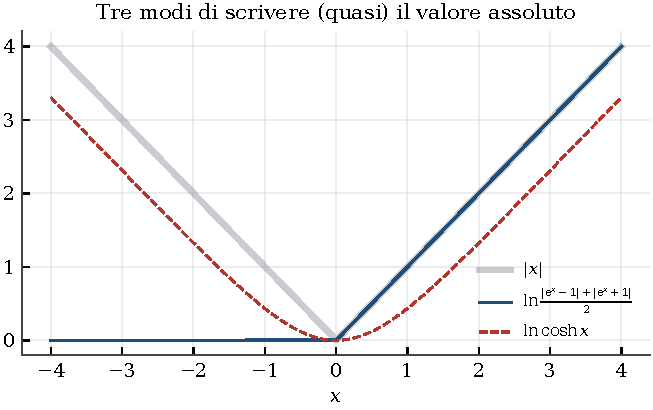
\includegraphics[width=0.86\linewidth]{../figures/mate_logcosh.pdf}
  \caption{Il meccanismo delle righe $\#77$--$\#81$: la media $\left(\left|\mathrm{e}^x-1\right|+\left|\mathrm{e}^x+1\right|\right)/2$ vale $\max\!\left(\mathrm{e}^x,1\right)$, e il suo logaritmo è $\max(x,0)$. Per confronto, $\ln\cosh x$ approssima $|x|$ ma non lo raggiunge mai.}
  \label{fig:mate_logcosh}
\end{figure}
\begin{espr}{82}{User}{}
\[
\frac{1}{2}\, \left(1 - \operatorname{sgn}\!\left(\sin\!\left(\pi\, \left(x - 1\right)\right)\right)\right)
\]
\end{espr}
Un'onda quadra costruita direttamente con la funzione segno.

\begin{espr}{83}{User}{}
\[
\frac{\ln\!\left(\frac{\left|\mathrm{e}^{\sin\!\left(\pi\, x\right)} - 1\right| + \left|\mathrm{e}^{\sin\!\left(\pi\, x\right)} + 1\right|}{2}\right)}{\sin\!\left(\pi\, x\right)}
\]
\end{espr}
Il gradino composto con il seno: onda quadra di periodo $2$.

\begin{espr}{84}{User}{}
\[
\frac{\ln\!\left(\frac{\left|\mathrm{e}^{\cos\!\left(\pi\, x\right)} - 1\right| + \left|\mathrm{e}^{\cos\!\left(\pi\, x\right)} + 1\right|}{2}\right)}{\cos\!\left(\pi\, x\right)}
\]
\end{espr}
Il gradino composto con il coseno: la stessa onda sfasata.


La chiave è l'identità $\frac{|u-1|+|u+1|}{2}=\max(|u|,1)$, vera per ogni reale $u$. Ponendo $u=\mathrm{e}^x$, che è sempre positivo, si ottiene $\max\left(\mathrm{e}^x,1\right)=\mathrm{e}^{\max(x,0)}$, e quindi
\[
  \frac{1}{x}\ln\frac{\left|\mathrm{e}^x-1\right|+\left|\mathrm{e}^x+1\right|}{2}
  =\frac{\max(x,0)}{x}
  =\begin{cases}1 & x>0\\ 0 & x<0.\end{cases}
\]
È il gradino di Heaviside, riga $\#77$. La riga $\#80$ raddoppia l'argomento e sottrae uno, ottenendo $2\max(x,0)/x-1=\mathrm{sgn}(x)$: è la funzione segno della riga $\#79$. La verifica numerica conferma entrambe esattamente. Le righe $\#83$ e $\#84$ compongono il gradino con seno e coseno e producono onde quadre.

\section{Onde triangolari e a dente di sega}

Il filone prosegue con le funzioni periodiche non sinusoidali, costruite componendo una funzione trigonometrica con l'inversa di un'altra. È il trucco che permette di ottenere spigoli da funzioni lisce.

\begin{espr}{85}{User}{}
\[
\operatorname{tri}\!\left(x\right)
\]
\end{espr}
La funzione triangolare predefinita di Derive, per confronto.

\begin{espr}{86}{User}{}
\[
\frac{1}{\pi}\, \arccos\!\left(\sin\!\left(\pi\, \left(x - \frac{1}{2}\right)\right)\right)
\]
\end{espr}
L'onda triangolare costruita con arcocoseno e seno.

\begin{espr}{87}{User}{}
\[
\left|\frac{2}{\pi}\, \arcsin\!\left(\cos\!\left(\frac{\pi\, x}{2}\right)\right)\right|
\]
\end{espr}
La stessa onda costruita con arcoseno e coseno: le due espressioni coincidono punto per punto.

\begin{espr}{88}{User}{}
\[
\left|\frac{2}{\pi}\, \arctan\!\left(\cot\!\left(\frac{\pi\, x}{2}\right)\right)\right|
\]
\end{espr}
Una terza variante con arcotangente e cotangente.

\begin{espr}{89}{User}{}
\[
\frac{4\, \arcsin^{2}\!\left(\cos\!\left(\frac{\pi\, x}{2}\right)\right)}{\pi\, \arcsin\!\left(\cos\!\left(\pi\, x\right)\right) + \frac{\pi^{2}}{2}}
\]
\end{espr}
Una combinazione quadratica delle precedenti.

\begin{espr}{90}{User}{}
\[
\operatorname{mod}\!\left(x\right)
\]
\end{espr}
La parte frazionaria secondo Derive.

\begin{espr}{91}{User}{}
\[
1 + \sum_{k=-\infty}^{+\infty} \frac{\mathrm{i}\, \mathrm{e}^{\mathrm{i}\, k\, \pi\, t}}{k\, \pi}
\]
\end{espr}
La serie di Fourier del dente di sega, in forma esponenziale bilatera.

\begin{espr}{92}{User}{}
\[
\frac{1}{\pi}\, \operatorname{arccot}\!\left(\tan\!\left(-\pi\, \left(x + \frac{1}{2}\right)\right)\right)
\]
\end{espr}
Il dente di sega costruito con arcocotangente e tangente.

\begin{espr}{93}{User}{}
\[
\frac{1}{\pi}\, \operatorname{arccot}\!\left(\tan\!\left(-\pi\, \left(x - \frac{1}{2}\right)\right)\right)
\]
\end{espr}
La stessa onda traslata di mezzo periodo.

\begin{figure}[htbp]
  \centering
  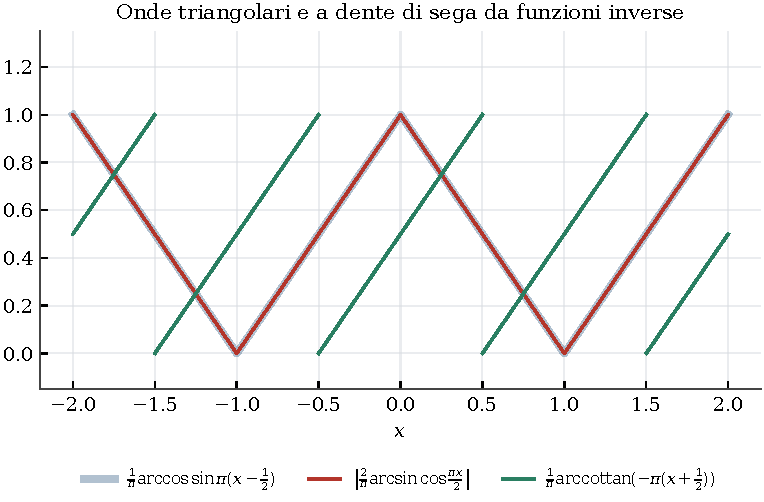
\includegraphics[width=0.86\linewidth]{../figures/mate_onde.pdf}
  \caption{Le tre costruzioni delle righe $\#86$, $\#87$ e $\#92$. Le prime due danno la stessa onda triangolare — la curva blu spessa è nascosta sotto la rossa — mentre la terza dà il dente di sega.}
  \label{fig:mate_onde}
\end{figure}
\begin{espr}{94}{User}{}
\[
-\log\!\left(\frac{1}{\pi}\, \operatorname{arccot}\!\left(\tan\!\left(\pi\, \left(x + \frac{1}{2}\right)\right)\right)\right)
\]
\end{espr}
Il logaritmo del dente di sega, cambiato di segno.

\begin{espr}{95}{User}{}
\[
-\log\!\left(\frac{1}{\pi}\, \arccos\!\left(\sin\!\left(\pi\, \left(x - \frac{1}{2}\right)\right)\right)\right)
\]
\end{espr}
L'analogo con l'onda triangolare.

\begin{espr}{96}{User}{}
\[
\arccos\!\left(\sin\!\left(-\log\!\left(\frac{1}{\pi}\, \arccos\!\left(\sin\!\left(\pi\, \left(x - \frac{1}{2}\right)\right)\right)\right)\right)\right)
\]
\end{espr}
Una composizione ulteriore.

\begin{espr}{97}{User}{}
\[
\frac{\sin\!\left(x\right)}{x}\, \left(\frac{1}{\pi}\, \operatorname{arccot}\!\left(\tan\!\left(-\pi\, \left(x + \frac{1}{2}\right)\right)\right)\right)
\]
\end{espr}
Il seno cardinale modulato dal dente di sega.

\begin{espr}{98}{User}{}
\[
\sin\!\left(\arccos\!\left(\arcsin\!\left(\cos\!\left(x + \frac{\pi}{2}\right)\right)\right)\right)
\]
\end{espr}
Una catena di funzioni inverse che si semplifica.

\begin{espr}{99}{User}{}
\[
\frac{\sin\!\left(x\right)}{x}\, \left(\frac{1}{\pi}\, \operatorname{arccot}\!\left(\tan^{2}\!\left(-\pi\, \left(x + \frac{1}{2}\right)\right)\right)\right)
\]
\end{espr}
Variante con il dente di sega al quadrato.

\begin{espr}{100}{User}{}
\[
\frac{4\, \arcsin^{2}\!\left(\cos\!\left(x\right)\right)}{\pi}\, \left(\arcsin\!\left(\cos\!\left(2\, x\right)\right) + \frac{\pi}{2}\right)
\]
\end{espr}
Una combinazione di arcoseni di coseni.

\begin{espr}{101}{User}{}
\[
\frac{2\, \arcsin\!\left(\cos^{2}\!\left(\frac{\pi\, x}{2}\right)\right)}{\arcsin\!\left(\cos\!\left(\pi\, x\right)\right) + \frac{\pi}{2}}
\]
\end{espr}
Un'altra, con argomenti dimezzati.

\begin{espr}{102}{Dif(\#94,x)}{}
\[
\frac{\mathrm{d}}{\mathrm{d}x}\!\left[-\log\!\left(\frac{1}{\pi}\, \operatorname{arccot}\!\left(\tan\!\left(\pi\, \left(x + \frac{1}{2}\right)\right)\right)\right)\right]
\]
\end{espr}
Si deriva la riga $\#94$.

\begin{espr}{103}{Simp(Dif(\#94,x))}{}
\[
\frac{1}{1 - \operatorname{mod}\!\left(x\right)}
\]
\end{espr}
Il risultato è $1/(1-\{x\})$: una funzione con asintoto verticale a ogni intero.


Le prime due costruzioni, $\#86$ e $\#87$, danno la stessa onda triangolare di periodo $2$ che vale $1$ sugli interi pari e $0$ su quelli dispari: si verifica punto per punto che coincidono. La riga $\#92$ dà invece il dente di sega, cioè la parte frazionaria, e la riga $\#90$ nomina la funzione che Derive usa allo stesso scopo.

La riga $\#91$ è la serie di Fourier del dente di sega, scritta in forma esponenziale complessa bilatera. Le righe $\#102$ e $\#103$ chiudono il filone in modo elegante: derivando il logaritmo del dente di sega si ottiene $1/(1-\{x\})$, dove $\{x\}$ è la parte frazionaria — una funzione che ha un asintoto verticale a ogni intero.

\section{Il dente di sega passa per il piano complesso}

Sette righe che rifanno la stessa costruzione con le funzioni iperboliche inverse, cioè spostandola sull'asse immaginario, e ne separano parte reale e parte immaginaria.

\begin{espr}{104}{User}{\verificata}
\begin{align*}
& \frac{2}{\pi}\, \operatorname{arcoth}\!\left(\tan\!\left(-\pi\, \left(x + \frac{1}{2}\right)\right)\right) \\
=\;& \frac{-2\, \mathrm{i}\, \operatorname{arccot}\!\left(-\mathrm{i}\, \cot\!\left(\pi\, x\right)\right)}{\pi}
\end{align*}
\end{espr}
La versione iperbolica del dente di sega, e la sua riscrittura come arcocotangente di argomento immaginario.

\begin{espr}{105}{User}{}
\[
\operatorname{Re}\!\left(\frac{-2\, \mathrm{i}\, \operatorname{arccot}\!\left(-\mathrm{i}\, \cot\!\left(\pi\, x\right)\right)}{\pi}\right)
\]
\end{espr}
Se ne chiede la parte reale.

\begin{espr}{106}{User}{\verificata}
\begin{align*}
& -\frac{\ln\!\left(\frac{1 - 2\, \sin\!\left(\pi\, x\right)\, \cos\!\left(\pi\, x\right)}{2\, \sin\!\left(\pi\, x\right)\, \cos\!\left(\pi\, x\right) + 1}\right)}{2\, \pi} \\
=\;& -\frac{\ln\!\left(\frac{1 - \sin\!\left(2\, \pi\, x\right)}{1 + \sin\!\left(2\, \pi\, x\right)}\right)}{2\, \pi}
\end{align*}
\end{espr}
Che vale un logaritmo di un rapporto in $\sin2\pi x$: due scritture equivalenti dello stesso risultato.

\begin{espr}{107}{User}{}
\[
-\operatorname{Im}\!\left(\frac{-2\, \mathrm{i}\, \operatorname{arccot}\!\left(-\mathrm{i}\, \cot\!\left(\pi\, x\right)\right)}{\pi}\right)
\]
\end{espr}
Se ne chiede la parte immaginaria, cambiata di segno.

\begin{espr}{108}{User}{}
\begin{align*}
& -\frac{\operatorname{sgn}\!\left(\sin\!\left(\pi\, x\right)\, \left(\cos\!\left(\pi\, x\right) + \sin\!\left(\pi\, x\right)\right)\right)}{2} - \frac{\operatorname{sgn}\!\left(\sin\!\left(\pi\, x\right)\, \left(\cos\!\left(\pi\, x\right) - \sin\!\left(\pi\, x\right)\right)\right)}{2} \\
&\qquad + 1
\end{align*}
\end{espr}
Che è una combinazione di funzioni segno: una scala a gradini.

\begin{espr}{109}{User}{\verificata}
\begin{align*}
& \frac{+\sin\!\left(\pi\, x\right)\, \left(\sin\!\left(\pi\, x\right) + \cos\!\left(\pi\, x\right)\right)}{2} + \frac{\sin\!\left(\pi\, x\right)\, \left(\sin\!\left(\pi\, x\right) - \cos\!\left(\pi\, x\right)\right)}{2} \\
&\qquad - \frac{1}{2} \\
=\;& \sin^{2}\!\left(\pi\, x\right) - \frac{1}{2}
\end{align*}
\end{espr}
Verifica algebrica intermedia.

\begin{espr}{110}{User}{\verificata}
\begin{align*}
& +\sin\!\left(\pi\, x\right)\, \left(\sin\!\left(\pi\, x\right) + \cos\!\left(\pi\, x\right)\right) + \sin\!\left(\pi\, x\right)\, \left(\sin\!\left(\pi\, x\right) - \cos\!\left(\pi\, x\right)\right) \\
&\qquad - 1 \\
=\;& 2\, \sin^{2}\!\left(\pi\, x\right) - 1 \\
=\;& -\cos\!\left(2\, \pi\, x\right)
\end{align*}
\end{espr}
La verifica completa: i termini misti si cancellano e resta $2\sin^2(\pi x)-1=-\cos(2\pi x)$.


La parte reale, riga $\#106$, è $-\frac{1}{2\pi}\ln\frac{1-\sin2\pi x}{1+\sin2\pi x}$: una funzione periodica con singolarità logaritmiche. La parte immaginaria, riga $\#108$, è una combinazione di funzioni segno, cioè una scala. La riga $\#110$ è l'unica identità algebrica esatta del gruppo e serve da verifica: sviluppando, $2\sin^2(\pi x)-1=-\cos(2\pi x)$.

\section{Quando una funzione iperbolica è anche circolare}

Quattro domande della stessa forma: esiste un $k$, eventualmente dipendente da $x$, per cui una funzione iperbolica coincide con la corrispondente circolare di argomento riscalato?

\begin{espr}{111}{User}{}
\[
\sinh\!\left(x\right) = \sin\!\left(k\, x\right)
\]
\end{espr}
Si chiede se il seno iperbolico coincida con un seno di argomento riscalato.

\begin{espr}{112}{User}{}
\[
k = \frac{\arcsin\!\left(\frac{\mathrm{e}^{x}}{2} - \frac{\mathrm{e}^{-x}}{2}\right)}{x}
\]
\end{espr}
Il fattore di scala esiste ma dipende da $x$.

\begin{espr}{113}{User}{}
\[
\cosh\!\left(x\right) = \cos\!\left(k\, x\right)
\]
\end{espr}
Stessa domanda per il coseno.

\begin{espr}{114}{Simp(Solve(\#113,k))}{}
\begin{align*}
& k = \frac{2\, \pi}{x} + \mathrm{i}\, \left(1 - \frac{\ln\!\left(\frac{\left|\mathrm{e}^{2\, x} - 1\right|}{2} + \frac{\mathrm{e}^{2\, x}}{2} + \frac{1}{2}\right)}{x}\right) \\[3pt]
\lor\quad & k = \mathrm{i}\, \left(1 - \frac{\ln\!\left(\frac{\left|\mathrm{e}^{2\, x} - 1\right|}{2} + \frac{\mathrm{e}^{2\, x}}{2} + \frac{1}{2}\right)}{x}\right) \\[3pt]
\lor\quad & k = \mathrm{i}\, \left(\frac{\ln\!\left(\frac{\left|\mathrm{e}^{2\, x} - 1\right|}{2} + \frac{\mathrm{e}^{2\, x}}{2} + \frac{1}{2}\right)}{x} - 1\right)
\end{align*}
\end{espr}
Le soluzioni sono immaginarie: $\cosh x\geq1$ e nessun coseno di argomento reale può eguagliarlo se non in $x=0$.

\begin{espr}{115}{User}{}
\[
\tanh\!\left(x\right) = \tan\!\left(k\, x\right)
\]
\end{espr}
Per la tangente.

\begin{espr}{116}{Simp(Solve(\#115,k))}{}
\begin{align*}
& k = \frac{\arctan\!\left(\frac{\mathrm{e}^{2\, x} - 1}{\mathrm{e}^{2\, x} + 1}\right)}{x} - \frac{\pi}{x} \\[3pt]
\lor\quad & k = \frac{\arctan\!\left(\frac{\mathrm{e}^{2\, x} - 1}{\mathrm{e}^{2\, x} + 1}\right)}{x} + \frac{\pi}{x} \\[3pt]
\lor\quad & k = \frac{\arctan\!\left(\frac{\mathrm{e}^{2\, x} - 1}{\mathrm{e}^{2\, x} + 1}\right)}{x}
\end{align*}
\end{espr}
Tre rami che differiscono per multipli di $\pi/x$: la tangente è periodica.

\begin{espr}{117}{User}{}
\[
\frac{\arctan\!\left(\frac{\mathrm{e}^{2\, x} - 1}{\mathrm{e}^{2\, x} + 1}\right)}{x}
\]
\end{espr}
Il ramo principale isolato.

\begin{espr}{118}{User}{}
\[
\operatorname{arcsinh}\!\left(x\right) = \arcsin\!\left(k\, x\right)
\]
\end{espr}
Per il seno iperbolico inverso.

\begin{espr}{119}{Simp(Solve(\#118,k))}{}
\begin{align*}
& k \\
=\;& \begin{cases} \frac{\sin\!\left(\ln\!\left(\sqrt{x^{2} + 1} + x\right)\right)}{x} & \text{se } -\frac{\pi}{2} < \ln\!\left(\sqrt{x^{2} + 1} + x\right) < \frac{\pi}{2} \end{cases}
\end{align*}
\end{espr}
Il caso più pulito: $k=\sin\!\left(\operatorname{arcsinh}x\right)/x$, con la condizione che tiene l'argomento nel dominio dell'arcoseno.

\begin{espr}{120}{User}{}
\[
\frac{\sin\!\left(\ln\!\left(\sqrt{x^{2} + 1} + x\right)\right)}{x}
\]
\end{espr}
Il fattore isolato.

\begin{espr}{121}{User}{}
\[
\operatorname{artanh}\!\left(x\right) = \arctan\!\left(k\, x\right)
\]
\end{espr}
Per la tangente iperbolica inversa.

\begin{espr}{122}{Simp(Solve(\#121,k))}{}
\begin{align*}
& k \\
=\;& \begin{cases} -\frac{\tan\!\left(\mathrm{i}\, \arctan\!\left(\mathrm{i}\, x\right)\right)}{x} & \text{se } -2\, \pi < \ln\!\left(\frac{\left(x - 1\right)^{2}}{\left(x + 1\right)^{2}}\right) < 2\, \pi \end{cases}
\end{align*}
\end{espr}
La soluzione, con la stessa struttura.

\begin{espr}{123}{User}{}
\[
\ln\!\left(\frac{\left(x - 1\right)^{2}}{\left(x + 1\right)^{2}}\right)
\]
\end{espr}
L'argomento del logaritmo che vi compare.


Le risposte sono tutte della forma $k=k(x)$, cioè il fattore di scala esiste ma non è costante. Il caso più pulito è $\#118$: da $\operatorname{arcsinh}x=\arcsin(kx)$ segue $kx=\sin\!\left(\operatorname{arcsinh}x\right)$ e quindi, essendo $\operatorname{arcsinh}x=\ln\!\left(x+\sqrt{x^2+1}\right)$, si ha $k=\sin\!\left(\ln\!\left(x+\sqrt{x^2+1}\right)\right)/x$: esattamente la risposta $\#119$, con la condizione che garantisce di restare nel dominio dell'arcoseno. Il caso $\#113$ mostra invece che per il coseno il fattore è necessariamente immaginario: $\cosh x\geq1$ e $\cos$ non può superare $1$ con argomento reale.

La risposta sistematica a queste domande è la funzione gudermanniana $\operatorname{gd}x=2\arctan\left(\tanh\tfrac x2\right)$, che lega funzioni circolari e iperboliche senza passare per i numeri complessi: $\tan(\operatorname{gd}x)=\sinh x$, $\sin(\operatorname{gd}x)=\tanh x$, $\cos(\operatorname{gd}x)=1/\cosh x$. Per esempio la soluzione principale della riga $\#116$, $kx=\arctan(\tanh x)$, vale $\tfrac12\operatorname{gd}(2x)$.

\section{Arcoseno e arcocoseno di argomento complesso}

Le ultime dieci righe tornano al piano complesso con due identità di conversione e alcune espressioni miste che il quaderno lascia aperte.

\begin{espr}{124}{User}{}
\[
\arcsin\!\left(z\right) + \mathrm{i}\, \arccos\!\left(z\right) = x + \mathrm{i}\, y
\]
\end{espr}
Si pone una combinazione di arcoseno e arcocoseno uguale a un numero complesso generico.

\begin{espr}{125}{User}{}
\[
z + \sin\!\left(\mathrm{i}\, \arccos\!\left(z\right)\right) = \sin\!\left(x + \mathrm{i}\, y\right)
\]
\end{espr}
Si applica il seno a entrambi i membri.

\begin{espr}{126}{User}{}
\[
\cos\!\left(\arcsin\!\left(z\right)\right) + \cos\!\left(\mathrm{i}\, \arccos\!\left(z\right)\right) = \cos\!\left(x + \mathrm{i}\, y\right)
\]
\end{espr}
E il coseno.

\begin{espr}{127}{User}{\verificata}
\[
\cos\!\left(\mathrm{i}\, \arccos\!\left(z\right)\right) = \cosh\!\left(-\arccos\!\left(z\right)\right)
\]
\end{espr}
La regola di conversione per il coseno di argomento immaginario.

\begin{espr}{128}{User}{\verificata}
\[
\sin\!\left(\mathrm{i}\, \arccos\!\left(z\right)\right) = \frac{1}{\mathrm{i}}\, \sinh\!\left(-\arccos\!\left(z\right)\right)
\]
\end{espr}
E per il seno, con il fattore $1/\mathrm{i}$.

\begin{espr}{129}{User}{\verificata}
\[
\sin\!\left(\mathrm{i}\, \arccos\!\left(z\right)\right) = \mathrm{i}\, \sinh\!\left(\arccos\!\left(z\right)\right)
\]
\end{espr}
La stessa riga scritta con $\mathrm{i}$ al numeratore: $1/\mathrm{i}=-\mathrm{i}$ e il segno dell'argomento si compensa.

\begin{espr}{130}{User}{}
\[
\mathrm{e}^{x} + \mathrm{i}\, \mathrm{e}^{y}
\]
\end{espr}
Un'espressione mista, punto di partenza per l'ultimo gruppo.

\begin{espr}{131}{Sub(User)}{}
\[
\pi\, \mathrm{e}^{\mathrm{i}\, \left(x + \mathrm{i}\, y\right)} + \mathrm{i}\, \mathrm{e}^{\pi\, \left(x + \mathrm{i}\, y\right)}
\]
\end{espr}
Con la sostituzione $x\to x+\mathrm{i}y$ e i due esponenziali scambiati di base.

\begin{espr}{132}{User}{\verificata}
\begin{align*}
& \pi\, \mathrm{e}^{-y + \frac{\mathrm{i}\, \left(2\, x + \pi\right)}{2}} + \pi\, \mathrm{e}^{\pi\, x}\, \left(-1\right)^{\frac{2\, y + 1}{2}} \\
=\;& -\mathrm{i}\, \left(-\pi\, \mathrm{e}^{-y + \mathrm{i}\, x} - \pi\, \mathrm{e}^{\pi\, x}\, \left(-1\right)^{y}\right)
\end{align*}
\end{espr}
L'identità che ne risulta, verificata da Derive.

\begin{espr}{133}{User}{}
\[
\frac{\ln\!\left(\frac{\left|\mathrm{e}^{x} - 1\right| + \left|\mathrm{e}^{x} + 1\right|}{2}\right)}{x}
\]
\end{espr}
L'ultima riga del quaderno ripete il gradino della riga $\#77$.


Le righe $\#127$--$\#129$ sono le regole di conversione: $\cos(\mathrm{i}w)=\cosh w$ e $\sin(\mathrm{i}w)=\mathrm{i}\sinh w$, scritte con $w=\arccos z$. L'ultima riga ripete testualmente la $\#77$: il quaderno si chiude tornando al gradino, che è forse il risultato di cui l'autore era più soddisfatto.

\section*{In sintesi}
\addcontentsline{toc}{section}{In sintesi}

Il quaderno vale soprattutto per due cose. La prima è l'identità di apertura, che è vera, elementare e ripresa una quarantina di volte: il rapporto fra differenze di quadrati di coseni e differenze di coseni duplicati è la costante $1/2$, e la versione con la triplicazione dà $1/4$; la regola $2^{1-n}$ vale solo per $n=2$ e $n=3$. La seconda è la costruzione del gradino e della funzione segno con soli logaritmi e valori assoluti, che è esatta: il gradino vale $\max(x,0)/x$, perché $\left(|\mathrm{e}^x-1|+|\mathrm{e}^x+1|\right)/2=\max(\mathrm{e}^x,1)$.

In mezzo c'è una lunga sezione dedicata a interrogare un'equazione indeterminata, con la sua risposta priva di significato inseguita per trenta espressioni. Averla conservata non toglie niente al resto: mostra come questi quaderni venissero usati davvero, cioè come strumenti per provare, non per esporre.

